\setRL
\clearpage
\pagenumbering{arabic} 



در این بخش تمام اطلاعات مدل‌سازی غشای لیپیدی را می‌نویسم.


\section{
بررسی مدل‌ها شبیه‌سازی غشای سلولی.
}
\subsection{
بیولوژی غشا و ساختار آن
}
\subsection{
بررسی مدل گومپر-کرول
}
همانند بخش‌های دیگر فیزیک مانند دینامیک شاره‌ها و نظریه‌ی رسانایی در فلزات، نظریه‌ی پوسته‌های نازک می‌خواهد فیزیک اختلال‌های کُند را بر حسب چند پارامتر ماکروسکوپیک بیان کند. البته که بارها نشان داده شده که چنین نظریه‌هایی به شکل‌ جالبی فروپاشی می‌کنند. مانند با توجه به نظریه جفت شدن مُود‌ها و نظریه باز به هنجارش، افت و خیز‌ها گرمایی باعث می‌شوند که وشکسانی برشی
\LTRfootnote{shear viscosity}
شاره‌های تراکم ناپذیر در ۲ بعد به صورت لوگاریتمی با افزایش اندازه سیستم به بی نهایت میل می‌کند 
\cite{gomppernelson2012}
. غیر خطی شدن رفتار در مورد پوسته‌ها و صفحه‌های نازک نیز اتفاق می‌افتد. افت و خیز گرمایی می‌توانند بر ساختار پوسته‌هایی میکرونی به شدت تاثیر بگذارند زیراکه انرژی خمشی لازم برای بیشتر تغییر شکل‌های پوسته‌های خیلی نازک که زخامت آنها در مقیاس نانومتر است، حدود $k_BT$ است که در اینجا $k_B$ ثابت بولتزمن و
$T$
دماست. مکانیک آماری غشاها و صفحات تخت در گذشته بسیار دقبق مورد مطالعه قرار گرفته. در این سیستم‌ها نشان داده شده‌است که افت و خیز گرمایی در غشاهای تخت باعث می‌شود که مدول کشسانی درون صفحه‌ای
\LTRfootnote{in-plane}
 تابع اندازه‌‌ی سیستم باشد و در اندازه‌های بزرگ به سمت صفر میل کند در حالی که مدول خمشی به بی‌نهایت میل می‌کند. این پدیده‌های ناهنجار ناشی از جفت شدگی غیر خطی میان تغییر شکل‌های خارج از صفحه‌ای (عمود بر صفحه) و تنش‌هایی داخل صفحه‌ی که ایجاد می‌کنند که هنگام تغییر شکل خارج از صفحه از مرتبه‌ی دوم هستند. حتی اطلاعات کمتری در مورد تاثیر افت و خیز گرمایی بر غشا‌های کروی موجود است (شکل 
 \ref{fig:mem1}
)
ولی جفت شدگی بین تغییر شکل‌های روی سطح و عمود بر سطح با یکدیگر تفاوت دارند. به علت وجود هندسه‌ی بسته‌ی غشاهای شبه کروی تغییر شکل حتما همراه با ایجاد کشش در سطح است. در نتیجه جابجایی عمود بر سطح به شکل جملات مرتبه‌ی اول در تنش موازی با صفحه ظاهر می‌شوند. در نتیجه جفت‌ شدگی‌های غیر خطی متفاوت با غشای تخت ایجاد می‌‌شود.

انرژی کشسانی تغییر شکل غشا به شعاع
 $R$ 
با نظریه‌ی پوسته‌های نازک کم عمق مدل‌سازی می‌شود. با این روی‌کرد صحبت از فرورفتیگی‌ها یا برآمدگی‌هایی است که نسبت به بخش مورد مطالعه کوچک هستند. جابجایی درون صفحه با فنون دو مولفه‌ای 
$u_i(\boldsymbol{x})$ 
پارمتری‌سازی شده و جابجایی‌های عمود بر سطح با میدان 
$f(\boldsymbol{x})$
در دستگاه مختصات
$\boldsymbol{x}=(x_1,x_2)$
موازی سطح تعریف می‌‌شود. ما فرض می‌کنیم که تمام غشای مورد بررسی دارای خواص کشسانی یکسان در همه جای سطح است در نتیجه می‌توانیم تاثیر ۱۲ نقطه نقصی که به ناچار بر روی سطح کره‌ی مثلث بندی شده ایجاد می‌شود را ناچیز در نظر بگیریم.
\subsection{میدان و تنش در نظریه پوسته‌ی کم عمق}
در این قسمت ما طبق روش کویتر
\LTRfootnote{Koiter}
و
\LTRfootnote{Heijden}
هیدن

پیش می‌‌رویم
\cite{Heijden2008WTK}
. بخشی از کره که دچار فرورفتگی کوچکی شده را در نظر می‌گیریم و دستگاه مختصات دکارتی 
$(x_1,x_2)$
را طوری تعریف می‌کنیم که در مبدا بر قسمت بدون ناهمواری از کره مماس است (شکل 
\ref{fig:nelson_figs1}
). در نتیجه مرکز کره بر روی محور 
$z$
خواهد بود. می‌توان کره را با فاصله نقاط آن از صفحه‌ی مختصات پارامتری سازی کرد:
\begin{equation}
Z(x_1,x_2) = R\left(1-\sqrt{1-\frac{x_1^2}{R^2}-\frac{x_2^2}{R^2}}\right)
\label{eq:nelsonS1}
\end{equation}
\begin{figure}[h]
\begin{center}
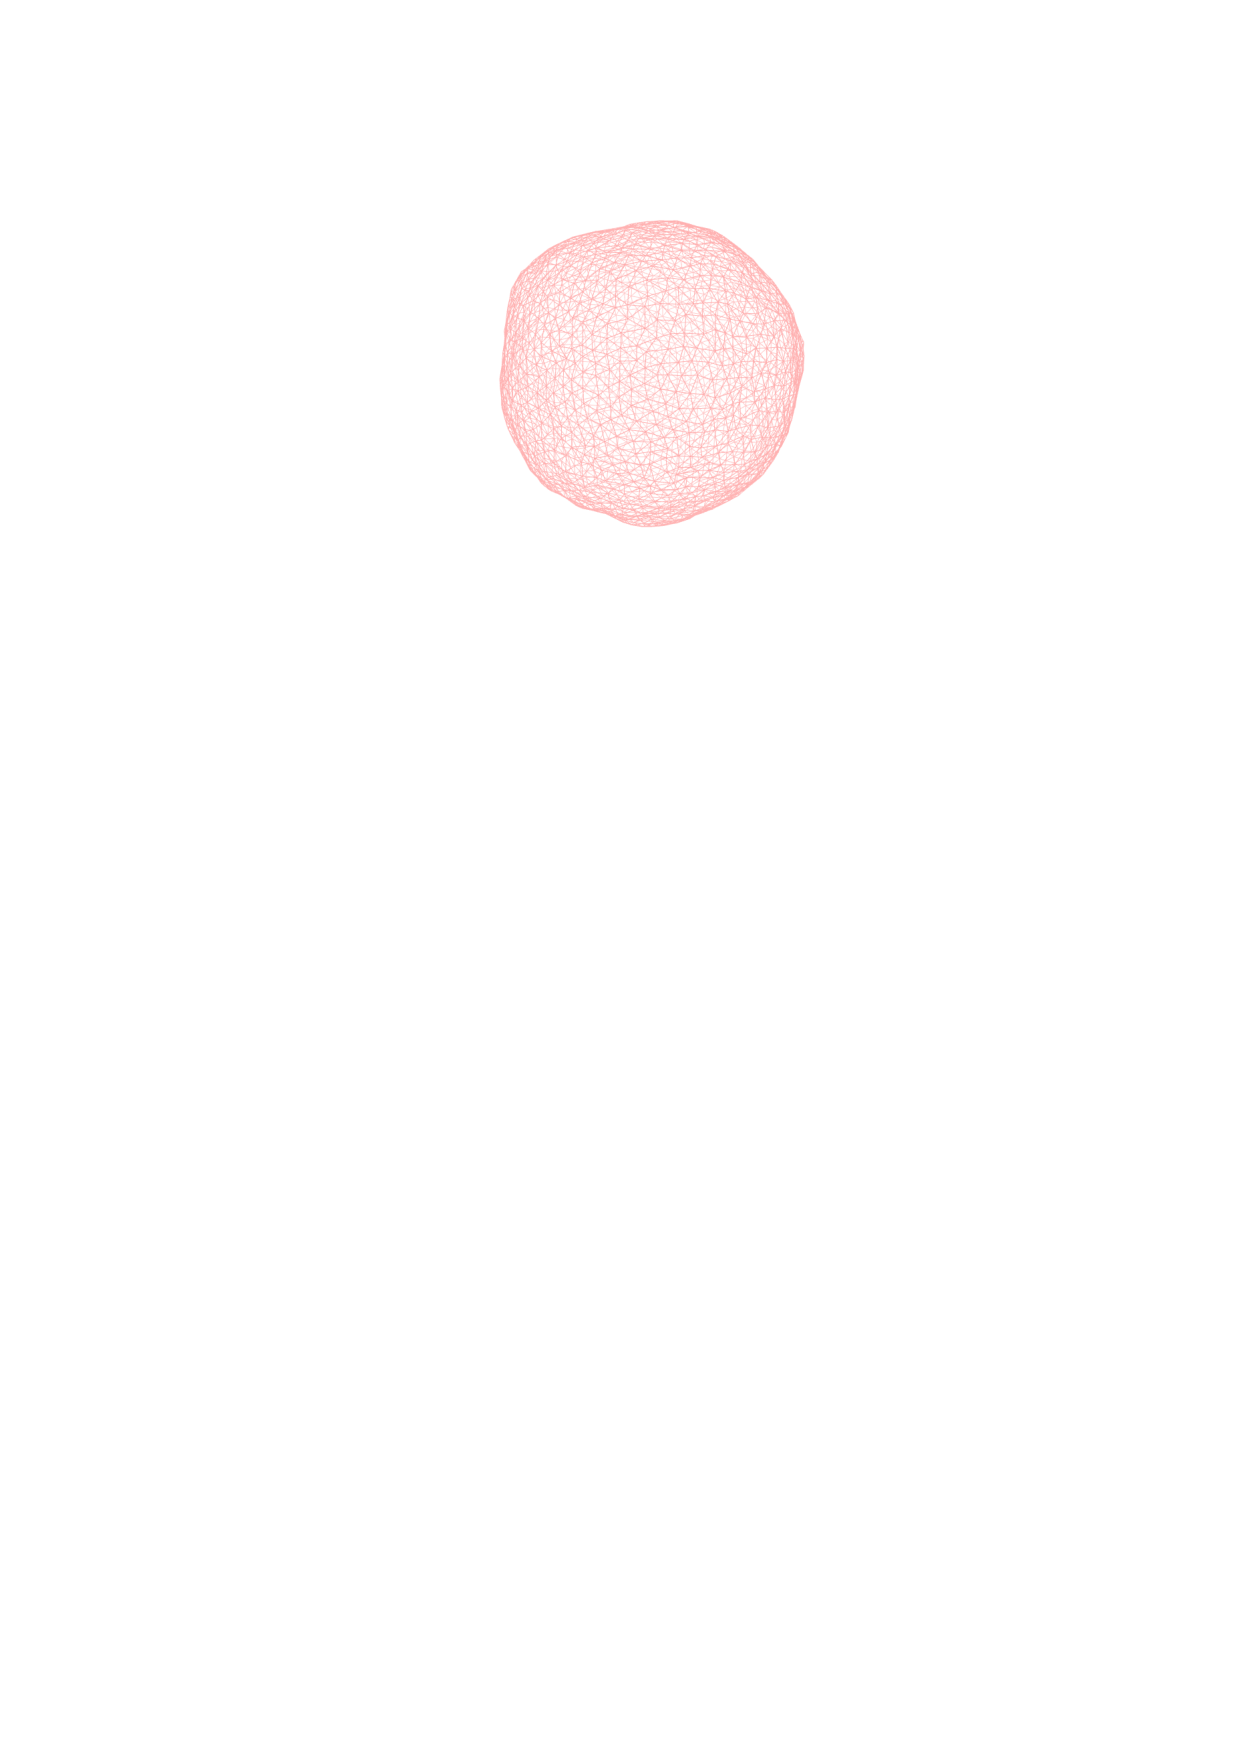
\includegraphics[width=4in]{mem_sim1}
\caption{
غشا با هندسه‌ی کروی.
}
\label{fig:mem1}
\end{center}
\end{figure}
\begin{figure}[h]
\begin{center}
\includegraphics[width=4in]{nelsons1}
\caption{
مبدا مختصات مماس به بخشی از کره‌ی بدون تغییر شکل.ٓ
}
\label{fig:nelson_figs1}
\end{center}
\end{figure}

که در اینجا 
$z=Z()z_1,x_2)$
نقاط روی کره در حالت بدون اختلال را مشخص می‌کند. در نظریه پوسته‌ی کم عمق فرض می‌شود که محل بررسی به اندازه‌ای کوچک است که شیب‌های 
$\partial_1Z\sim x_1/R$
و 
$\partial_2Z\sim x_2/R$
اندازه‌گیری شده نسبت به صفحه‌ی 
$(x_1,x_2)$
کوچک هستند. در نتیجه می‌توان معادله‌ی بالا رو به شکل زیر ساده کرد:
\begin{equation}
Z(x_1,x_2) \approx \frac{x_1^2+x_2^2}{2R}
\label{eq:nelsonS2}
\end{equation}
در نتیجه تمام تغییر شکل‌های پوسته از این حالت را می‌توان بر حسب جابجایی‌های عمود بر صفحه‌
 $f(x_1,x_2)$
و جابجایی های مماس بر صفحه 
$u_1(x_1,x_2)$
و
$u_2(x_1,x_2)$
که به ترتیب جابجایی در راستای محورهای 
$x_1$
و
$x_2$
را مشخص می‌کنند، تعریف کرد. بنابراین با توجه به میدان‌های تعریف شده، نقطه‌ی 
$(x_1,x_2,Z(x_1,x_2))$
در حالت بدون جابجایی در مرتبه‌ی اول به نقطه‌ی 
$(x_1+u_1-f\partial_1Z,x_2+u_2-f\partial_2Z,Z+f)$
منتقل می‌شود که در اینجا 
$\partial_iZ=x_i/R$
است. تانسور کرنش با توجه رابطه‌ی میان اندازه‌ی یک عنصر خط در حالت تغییر حالت داده شده
$ds'$
و خط متناظر آن در حالت کاملا کروی تعریف می‌شود:
\begin{equation}
(ds')^2=ds^2+2u_{ij}dx_idx_j
\label{eq:nelsonS3}
\end{equation}
در نتیجه با صرف نظر از مشتق‌های مرتبه‌های بالاتر می‌توان تانسور کرنش را تعریف کرد،
\begin{equation}
u_{ij}=\frac{1}{2}(\partial_iu_j+\partial_ju_i+\partial_if\partial_jf)-\delta_{ij}\frac{f}{R}
\label{eq:nelsonS4}
\end{equation}
در نتیجه انرژی کششی به شکل زیر تعریف خواهد شد
\begin{equation}
G_s=\frac{1}{2}\int dS\left[2\mu u_{ij}^2+\lambda u_{kk}^2\right]
\label{eq:nelsonS5}
\end{equation}
  که در اینجا 
$\lambda$
و
$\mu$
ضرایب لامه
\LTRfootnote{Lamé}
بوده و 
$dS$
عنصر مساحت است. همچنین انرژی هلفریش
\LTRfootnote{Helfrish}
را نیز در برای تغییرات خمشی پوسته در نظر می‌گیریم
\cite{Helfrich1973}.
\begin{equation}
G_b=\frac{1}{2}\int dS\left[\kappa(H-H_0)^2+\bar\kappa K\right]
\label{eq:nelsonS6}
\end{equation}
  که در اینجا 
$\kappa$
سختی خمشی، 
$H$
خمش متوسط (یا رد
\LTRfootnote{trace}
تانسور خمش)،
$H_0$
خمش ذاتی غشا،
$\bar\kappa$
مدول خمشی زینی،
و
$K$
دترمینان تانسور خمش است . با توجه به نظریه گاوس و بونه
\LTRfootnote{Gauss-Bonnet}
این انتگرال فقط یک عدد ثابت است که به انرژی آزاد سیستم اضافه می‌شود. در نتیجه از الان به بعد آن را در نظر نمی‌گیریم. همچنین فرض می‌کنیم که غشا خمش ذاتی ندارد. در نتیجه در قسمت کم عمق پوسته خمش موضعی بر حسب 
$Z(x_1,x_2)$
و 
$f(x_1,x_2)$
به شکل زیر محاسبه می‌شود:
\cite{Helfrich1973}.
\begin{equation}
H =\nabla^2(Z+f)=\frac{2}{R}+\nabla^2f
\label{eq:nelsonS7}
\end{equation}
که 
$\nabla^2=\partial_{11}+\partial_{22}$
لاپلاسین در دستگاه مختصات تعریف شده است. و در نهایت کار ناشی از فشار خارجی به صورت زیر تعریف می‌شود،
\cite{Helfrich1973}.
\begin{equation}
W=-p\int dSf
\label{eq:nelsonS8}
\end{equation}

و در نهایت با توجه به تقریب نظریه عنصر سطح به شکل زیر تعریف می‌شود،
\cite{Helfrich1973}.
\begin{equation}
dS=dx_1dx_2/\sqrt{1-(x_1^2+x_2^2)/R^2}\approx dx_1dx_2
\label{eq:nelsonS8.1}
\end{equation}







\begin{equation}
\begin{aligned}
\sigma=\sigma(t_1)+\sigma(t_2) \\
\gamma=\gamma(t_1)+\gamma(t_2)
\end{aligned}
\end{equation}

%\renewcommand{\refname}{whatever}
%\bibliography{reference} 
%\bibliographystyle{IEEEtran}
%\renewcommand\refname{مراجع}


	        
	       